\documentclass[aspectratio=169,11pt]{beamer}
\usepackage{../assets/agrawal-beamer}

\title[Agrawal et al. (2025)]{The Economics of Bicycles for the Mind}
\subtitle{Modelo, proposiciones y auditoría de la varianza}
\author{Belén Vásquez}
\institute{Universidad del Pacífico}
\date{Agosto de 2026}

\begin{document}

% 1
\begin{frame}[plain]
  \titlepage
  \vspace{-0.8em}
  \begin{center}\small
    \paperref\\[0.45em]
    \href{\RepoURL}{\texttt{github.com/sbvasquezg-ux/ai-02-agrawal}}
  \end{center}
\end{frame}

% 2
\begin{frame}{La herramienta eleva productividad, pero redistribuye capacidades}
  \textbf{Tensión.} Computadoras e IA hacen más barata la implementación, pero
  vuelven más valioso el juicio que decide \emph{qué} mejorar.

  \medskip
  \begin{enumerate}
    \item Modelo: cadena de mejoras y elección de esfuerzo.
    \item Proposiciones 1--2: esfuerzo, productividad y adopción.
    \item Proposición 3: heterogeneidad y varianza salarial.
    \item Auditoría: objeto correcto, condición faltante y dominio interior.
  \end{enumerate}

  \keybox{\textbf{Mensaje central.} La forma de U no es ``varianza de la IA'':
  es una propiedad condicional de $\operatorname{Var}[V_i(\theta)]$ dentro de
  una especialización y un rango interior.}
  \sourcefoot{\paperref, introducción y secciones 3--4.}
\end{frame}

% 3
\begin{frame}{CAD y predicción separan dos tipos de juicio}
  \begin{columns}[T,onlytextwidth]
    \column{0.48\textwidth}
    \begin{block}{CAD: encontrar mejoras}
      La computadora acelera cálculos y visualización. El trabajador puede
      iterar más, pero todavía debe identificar qué aspecto del diseño mejorar.

      \medskip
      \textbf{Capacidad clave:} juicio de oportunidad $\gamma(t)$.
    \end{block}
    \column{0.48\textwidth}
    \begin{block}{Predicción con IA: actuar bien}
      Una mejor predicción revela el estado, pero el decisor debe conocer la
      acción adecuada y capturar su valor.

      \medskip
      \textbf{Capacidad clave:} juicio de resultado $\alpha$.
    \end{block}
  \end{columns}
  \medskip
  \centering
  \textbf{Ambos ejemplos comparten implementación $s$ y esfuerzo $e$.}
  \sourcefoot{\paperref, sección 2.}
\end{frame}

% 4
\begin{frame}{El agente elige esfuerzo, no oportunidades ni capacidades}
  Condicional en encontrar una oportunidad:
  \[
  e_t^*(\theta)\in\arg\max_{e_t\ge0}
  \underbrace{\alpha\Delta p(se_t;\theta)-c(e_t;\theta)}_{M(e_t;\theta)}.
  \]
  \begin{itemize}
    \item Variable de elección: esfuerzo de implementación $e_t$.
    \item Restricción: $e_t\ge0$; $p(se_t;\theta)\in[0,1]$.
    \item Tecnología: $p$ creciente y cóncava; $c$ creciente y convexa.
    \item FOC interior: $\alpha\Delta s p'(se_t^*;\theta)=c'(e_t^*;\theta)$.
  \end{itemize}
  \sourcefoot{\paperref, ecuaciones (18)--(20).}
\end{frame}

% 5
\begin{frame}{Una herramienta mejora niveles, pero sustituye esfuerzo al margen}
  Para todo $e$ y $\theta'>\theta$, una herramienta cognitiva satisface
  \[
    p(se;\theta')\ge p(se;\theta),\qquad
    c(e;\theta')\le c(e;\theta),
  \]
  y
  \[
    \frac{p'(se;\theta)}{c'(e;\theta)}
    \quad\text{cae estrictamente con }\theta\text{ para }e>0.
  \]
  \keybox{La primera condición desplaza el beneficio neto hacia arriba; la
  segunda reduce el incentivo marginal a aportar esfuerzo humano.}
  \sourcefoot{\paperref, Definición 1.}
\end{frame}

% 6
\begin{frame}{Proposición 1: la herramienta reduce esfuerzo y eleva valor}
  \begin{block}{Resultado}
  Al pasar de $\theta=0$ a $\theta=1$:
  \begin{enumerate}
    \item $e_t^*(1)<e_t^*(0)$ en cada período;
    \item $e_t^*(\theta)=e^*(\theta)$ para rondas tecnológicamente idénticas;
    \item $V_0(1)>V_0(0)$.
  \end{enumerate}
  \end{block}
  \medskip
  \begin{block}{Intuición de la prueba}
    La caída de $p'/c'$ desplaza el cruce marginal hacia menor esfuerzo; la
    mejora de niveles eleva el máximo de $M$, que luego se suma sobre todas las
    oportunidades.
  \end{block}
  \sourcefoot{\paperref, Proposición 1 y Apéndice A.1.}
\end{frame}

% 7
\begin{frame}{La ganancia por ronda se amplifica por oportunidades futuras}
  Defina
  \[
  \Gamma=\sum_{t\ge0}\left(\prod_{i=0}^{t}\gamma(i)\right)\delta^t.
  \]
  Entonces
  \[
  V_0(1)-V_0(0)
  =\Gamma\,[M(e^*(1);1)-M(e^*(0);0)]>0.
  \]
  \keybox{$\Gamma$ no es productividad de implementación: es el número
  descontado de oportunidades que permite reutilizar la mejora de cada ronda.}
  \sourcefoot{\paperref, Proposición 2(1).}
\end{frame}

% 8
\begin{frame}{Proposición 2: cuatro comparativas ordenan la ganancia}
  \small
  \begin{block}{Resultado}
  \begin{enumerate}
    \item \textbf{Oportunidades:} mayor $\Gamma$ multiplica la ganancia.
    \item \textbf{Juicio de resultado:} la ganancia aumenta con $\alpha$ sii
      $p(se^*(1);1)\ge p(se^*(0);0)$.
    \item \textbf{Implementación:} el paper obtiene menor ganancia con $s$ si
      herramienta y habilidad son sustitutas.
    \item \textbf{Momento:} las oportunidades tempranas suelen pesar más por
      descuento, condicionadas por la secuencia completa.
  \end{enumerate}
  \end{block}
  \keybox{\small Dos cautelas: $p_{s\theta}<0$ a esfuerzo fijo no firma por sí
  sola la comparación entre óptimos; y $\partial\Gamma/\partial\gamma(t)$ debe
  incluir todos los términos futuros $k\ge t$.}
  \sourcefoot{\paperref, Proposición 2 y Apéndice A.2; auditoría propia.}
\end{frame}

% 9
\begin{frame}{La sección de desigualdad impone una especialización fuerte}
  \begin{itemize}
    \item $p(se;\theta)=\sqrt{se+\theta}$ y $c(e)=e$.
    \item $\gamma(0)=\gamma_0$ y $\gamma(t)=\gamma$ para $t>0$.
    \item $\alpha,\gamma_0,\gamma,s$ independientes, con soporte positivo.
    \item $\mu_i>3\sigma_i$ y momentos requeridos finitos.
    \item $\delta\gamma<1$ y $\Gamma=\gamma_0/(1-\delta\gamma)$.
    \item Rango común donde $e_i^*(\theta)>0$ para todos.
  \end{itemize}
  \keybox{La Proposición 3 no es un teorema general sobre cualquier IA: vive
  dentro de esta tecnología y de la región interior.}
  \sourcefoot{\paperref, sección 4, pp. 17--18.}
\end{frame}

% 10
\begin{frame}{La forma cerrada separa base, herramienta y oportunidades}
  \begin{align*}
  e^*(\theta)&=\frac{\alpha^2\Delta^2s}{4}-\frac{\theta}{s},\\
  M(\theta)&=\frac{\alpha^2\Delta^2s}{4}+\frac{\theta}{s},\\
  V(\theta)&=\Gamma\left(\frac{\alpha^2\Delta^2s}{4}+\frac{\theta}{s}\right).
  \end{align*}
  \begin{block}{Límite interior individual}
  \[
  e^*(\theta)>0
  \quad\Longleftrightarrow\quad
  \theta<\frac{\alpha^2\Delta^2s^2}{4}.
  \]
  \end{block}
  \sourcefoot{\paperref, ecuaciones (58)--(60); condición interior corregida.}
\end{frame}

% 11
\begin{frame}{Proposición 3 corregida: la U requiere heterogeneidad acotada}
  \small
  \begin{block}{Resultado}
  Bajo los supuestos mantenidos y $\operatorname{Var}(\Gamma/s)>0$:
  \begin{enumerate}
    \item $d\mathbb E[V(\theta)]/d\theta>0$.
    \item Si
      \[
      \frac{\mathbb E[\Gamma^2]}{\mathbb E[\Gamma]^2}
      <\mu_s\mathbb E[1/s],
      \]
      la varianza cae inicialmente y es estrictamente convexa.
    \item Existe un mínimo único $\theta^*>0$; la varianza aumenta para
      $\theta>\theta^*$.
    \item Pendiente positiva en $\theta=1$ exige además $\theta^*<1$.
  \end{enumerate}
  \end{block}
  \sourcefoot{\paperref, Proposición 3; corrección propia de (32).}
\end{frame}

% 12
\begin{frame}{La media sube; la varianza combina dos fuerzas}
  \[
  \frac{d\mathbb E[V(\theta)]}{d\theta}
  =\mathbb E[\Gamma]\mathbb E[1/s]>0.
  \]
  Como $V=\Gamma M$ y $\Gamma\perp M$,
  \[
  \operatorname{Var}(V)=\mathbb E[\Gamma^2]\operatorname{Var}(M)
  +\operatorname{Var}(\Gamma)\mathbb E[M]^2.
  \]
  \begin{itemize}
    \item $\theta/s$ favorece más a quienes tienen menor $s$: fuerza igualadora.
    \item $\Gamma$ multiplica el valor de cada mejora: fuerza desigualadora.
  \end{itemize}
  \sourcefoot{\paperref, ecuaciones (31), (34) y (64).}
\end{frame}

% 13
\begin{frame}{El punto de giro existe, pero puede estar después de uno}
  \[
  \frac{d}{d\theta}\operatorname{Var}[V(\theta)]
  =a_0+2\theta\operatorname{Var}(\Gamma/s),
  \]
  \[
  \theta^*=-\frac{a_0}{2\operatorname{Var}(\Gamma/s)}>0.
  \]
  \begin{columns}[T,onlytextwidth]
    \column{0.48\textwidth}
    \keybox{Condición (30) $\Longleftrightarrow a_0<0$: pendiente inicial
    negativa.}
    \column{0.48\textwidth}
    \keybox{Pendiente en uno positiva $\Longleftrightarrow\theta^*<1$: condición
    adicional.}
  \end{columns}
  \sourcefoot{\paperref, Apéndice A.3, ecuaciones (81)--(90).}
\end{frame}

% 14
\begin{frame}{Las tres preguntas del profesor tienen respuestas distintas}
  \small
  \begin{enumerate}
    \item \textbf{¿Varianza de qué y respecto de qué?} Varianza transversal de
      $V_i(\theta)$ (interpretada como salario) respecto de calidad $\theta$.
    \item \textbf{¿Es incondicional?} No. Requiere tecnología especializada,
      independencia, soporte, interioridad, (30) y
      $\operatorname{Var}(\Gamma/s)>0$.
    \item \textbf{¿Beneficio individual?}
      \[
      \operatorname{Var}[V(\theta)-V(0)]
      =\theta^2\operatorname{Var}(\Gamma/s),
      \]
      que crece monótonamente.
  \end{enumerate}
  \sourcefoot{Derivación propia a partir de \paperref, sección 4 y Apéndice A.3.}
\end{frame}

% 15
\begin{frame}{Tres slips separan el enunciado de lo demostrado}
  \small
  \begin{enumerate}
    \item \textbf{Ecuación (32):} (30) no implica pendiente positiva en uno;
      falta $\theta^*<1$.
    \item \textbf{Interioridad:} el paper usa $\Delta>2/(s\sqrt\alpha)$, pero
      la condición real es $\alpha^2\Delta^2s^2>4\theta$.
    \item \textbf{Dominio:} $\sqrt{se+\theta}$ puede exceder uno aunque $p$ sea
      probabilidad; para $\theta$ alto aparece $e^*=0$.
  \end{enumerate}
  \medskip
  \textbf{Vacíos adicionales en Prop. 2:} el efecto temporal omite sumandos
  futuros en el enunciado y la sustitución a esfuerzo fijo no garantiza la
  comparación entre óptimos.
  \sourcefoot{Auditoría algebraica propia; detalles en extensions.md.}
\end{frame}

% 16
\begin{frame}{SymPy confirma el álgebra y un contraejemplo interior}
  \begin{columns}[T,onlytextwidth]
    \column{0.58\textwidth}
    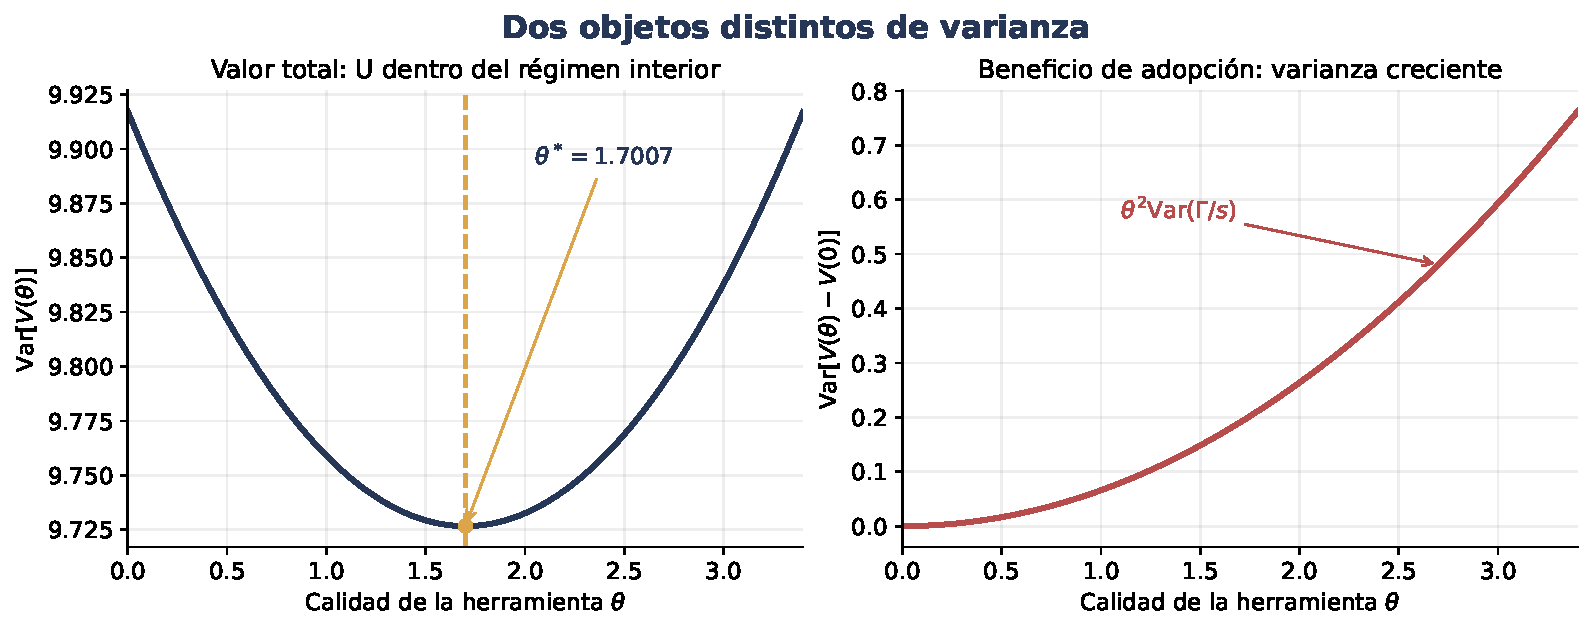
\includegraphics[width=\linewidth]{figures/variance-comparison.pdf}
    \column{0.39\textwidth}
    \small
    Uniformes independientes satisfacen (30):
    \[
      1.022930<1.031732.
    \]
    Pero
    \[
      \begin{aligned}
      \theta^*&=1.7007,\\
      \operatorname{Var}'[V(1)]&=-0.09239.
      \end{aligned}
    \]
    El límite interior común es $4.5574>\theta^*$.

    \keybox{La U existe, pero todavía está descendiendo en $\theta=1$; la
    varianza del beneficio de adopción crece desde cero.}
  \end{columns}
  \sourcefoot{sim.py; cuadratura Gauss--Legendre y SymPy.}
\end{frame}

\end{document}
